%%%%%%%%%%%%%%%%%%%%%%%%%%%%%%%%%%%%%%%%%%%%%%%%%%%%%%%%%%%%%%%%%%%%%%%%%%%%%%%%%%%%%%%%%%%%%%%%%%%%%%%%%%%%%%%%%%
%% Projeto de doutorado -- GAS UFSC -- Tex/LaTex
%% Autor: Eduardo Alberto Duarte Lacerda
%% Orientador: Roberto Cid Fernandes Jr.
%% 1a. parte: 27 maio 2014
%%%%%%%%%%%%%%%%%%%%%%%%%%%%%%%%%%%%%%%%%%%%%%%%%%%%%%%%%%%%%%%%%%%%%%%%%%%%%%%%%%%%%%%%%%%%%%%%%%%%%%%%%%%%%%%%%%
\documentclass[a4paper,12pt]{article}

\usepackage[utf8x]{inputenc}
\usepackage[portuguese,brazilian]{babel}
\usepackage[round,authoryear]{natbib}
\usepackage{aecompl}
\usepackage[table, usenames, dvipsnames]{xcolor}
\usepackage{color}
\usepackage{textcomp}
\usepackage{ctable}
\usepackage[T1]{fontenc}
\usepackage{mathrsfs}
%\PassOptionsToPackage{svgnames}{xcolor}
%\usepackage{listings}
%\usepackage{pdfpages}
\usepackage[colorlinks,linkcolor=black,bookmarks=true,citecolor=black]{hyperref}

%%% page geometry %%% 
\usepackage{geometry}
\geometry{verbose,a4paper,tmargin=3cm,bmargin=2.5cm,
lmargin=2.5cm,rmargin=2cm,headsep=5mm,footskip=0cm}

%%%% page layout %%%%
\usepackage{fancyhdr}
\pagestyle{fancy}
\lhead{}\chead{}\rhead{}
\lfoot{}\cfoot{}\rfoot{}
\fancyhead{}
\rfoot{\thepage}

\newcommand{\mnras}{MNRAS}
\newcommand{\apj}{ApJ}
\newcommand{\pasp}{PASP}
\renewcommand{\it}{\textit}
\newcommand{\aj}{AJ}					%{The Astronomical Journal}
\newcommand{\apjs}{ApJS}

%\renewcommand{\footrulewidth}{.5pt}
\renewcommand{\headrulewidth}{0.0pt}
%\documentclass{nathesis}
\usepackage{xspace}
\usepackage{color}
\usepackage{float}

% ********************* Lacerda's Definitions ************************
\newcommand\pycasso{\textsc{p}y\textsc{casso}\xspace}
%\newcommand\pcalifa{\textsc{pca}lifa\xspace}
\newcommand\pcalifa{PCA\textsc{lifa}\xspace}
\newcommand{\meanL}[1]{\relax\ifmmode \langle #1 \rangle_L \else $\langle #1 \rangle_L$\xspace \fi}
\newcommand{\mean}[1]{\relax\ifmmode \langle #1 \rangle \else $\langle #1 \rangle$\xspace \fi}
%*******************************************************************

% ********************* Andre's Definitions ************************
\def\starlight{\textsc{starlight}\xspace}      %smallcaps Starlight%
\def\starlightUV{\textsc{starlight+UV}\xspace} %smallcaps Starlight+UV%
\def\STARLIGHT{\textit{STARLIGHT}\xspace}                %Starlight%
\def\STARLIGHTUV{\textit{STARLIGHT+UV}\xspace}        %Starlight+UV%
%\def\SDSS{\textit{SDSS}\xspace}           %Sloan Digital Sky Survey%
\def\SDSS{SDSS\xspace}           %Sloan Digital Sky Survey%
\def\galex{\textit{GALEX}\xspace}
\def\citneed{\textsuperscript{\bf \textcolor{red}{[citation needed]}}\xspace}
\def\fixme{\textsuperscript{\bf \textcolor{red}{[FIXME]}}\xspace}
\def\Halpha{\ifmmode \mathrm{H}\alpha \else H$\alpha$\xspace \fi}
\def\WHa{\ifmmode W_{\mathrm{H}\alpha} \else $W_{\mathrm{H}\alpha}$\xspace \fi}
\def\Hbeta{\ifmmode \mathrm{H}\beta \else H$\beta$\xspace \fi}
\def\NII{[N\thinspace\textsc{ii}] $\lambda 6584$\xspace} 
\def\nII{\ifmmode [\mathrm{N\,\textsc{ii}}] \else [N\thinspace\textsc{ii}]\xspace \fi}
\def\WnII{W_{\mathrm{[N\,\textsc{ii}]}}}
\def\OIII{[O\thinspace\textsc{iii}] $\lambda 5007$\xspace}
\def\oIII{\ifmmode [\mathrm{O\,\textsc{iii}}] \else [O\thinspace{\sc iii}]\xspace \fi}
%*******************************************************************
% I guess these are Cid's definitions. I have found them in Luis'
% masters thesis. Some of them are rather useful.
% ********************* CID'S DEFINITIONS **************************

\def\ojo{\fbox{\bf !$\odot$j$\odot$!}}      %Olho! Needs Correction%

%*******************************************************************

% Journals - from AASTex
% Natalia@UFSC - 16/Nov/2005
\def\aj{AJ}%
          % Astronomical Journal
\def\actaa{Acta Astron.}%
          % Acta Astronomica
\def\araa{ARA\&A}%
          % Annual Review of Astron and Astrophys
\def\apj{ApJ}%
          % Astrophysical Journal
\def\apjl{ApJ}%
          % Astrophysical Journal, Letters
\def\apjs{ApJS}%
          % Astrophysical Journal, Supplement
\def\ao{Appl.~Opt.}%
          % Applied Optics
\def\apss{Ap\&SS}%
          % Astrophysics and Space Science
\def\aap{A\&A}%
          % Astronomy and Astrophysics
\def\aapr{A\&A~Rev.}%
          % Astronomy and Astrophysics Reviews
\def\aaps{A\&AS}%
          % Astronomy and Astrophysics, Supplement
\def\azh{AZh}%
          % Astronomicheskii Zhurnal
\def\baas{BAAS}%
          % Bulletin of the AAS
\def\caa{Chinese Astron. Astrophys.}%
          % Chinese Astronomy and Astrophysics
\def\cjaa{Chinese J. Astron. Astrophys.}%
          % Chinese Journal of Astronomy and Astrophysics
\def\icarus{Icarus}%
          % Icarus
\def\jcap{J. Cosmology Astropart. Phys.}%
          % Journal of Cosmology and Astroparticle Physics
\def\jrasc{JRASC}%
          % Journal of the RAS of Canada
\def\memras{MmRAS}%
          % Memoirs of the RAS
\def\mnras{MNRAS}%
          % Monthly Notices of the RAS
\def\na{New A}%
          % New Astronomy
\def\nar{New A Rev.}%
          % New Astronomy Review
\def\pra{Phys.~Rev.~A}%
          % Physical Review A: General Physics
\def\prb{Phys.~Rev.~B}%
          % Physical Review B: Solid State
\def\prc{Phys.~Rev.~C}%
          % Physical Review C
\def\prd{Phys.~Rev.~D}%
          % Physical Review D
\def\pre{Phys.~Rev.~E}%
          % Physical Review E
\def\prl{Phys.~Rev.~Lett.}%
          % Physical Review Letters
\def\pasa{PASA}%
          % Publications of the Astron. Soc. of Australia
\def\pasp{PASP}%
          % Publications of the ASP
\def\pasj{PASJ}%
          % Publications of the ASJ
\def\qjras{QJRAS}%
          % Quarterly Journal of the RAS
\def\rmxaa{Rev. Mexicana Astron. Astrofis.}%
          % Revista Mexicana de Astronomia y Astrofisica
\def\skytel{S\&T}%
          % Sky and Telescope
\def\solphys{Sol.~Phys.}%
          % Solar Physics
\def\sovast{Soviet~Ast.}%
          % Soviet Astronomy
\def\ssr{Space~Sci.~Rev.}%
          % Space Science Reviews
\def\zap{ZAp}%
          % Zeitschrift fuer Astrophysik
\def\nat{Nature}%
          % Nature
\def\iaucirc{IAU~Circ.}%
          % IAU Cirulars
\def\aplett{Astrophys.~Lett.}%
          % Astrophysics Letters and Communications
\def\apspr{Astrophys.~Space~Phys.~Res.}%
          % Astrophysics Space Physics Research
\def\bain{Bull.~Astron.~Inst.~Netherlands}%
          % Bulletin Astronomical Institute of the Netherlands
\def\fcp{Fund.~Cosmic~Phys.}%
          % Fundamental Cosmic Physics
\def\gca{Geochim.~Cosmochim.~Acta}%
          % Geochimica Cosmochimica Acta
\def\grl{Geophys.~Res.~Lett.}%
          % Geophysics Research Letters
\def\jcp{J.~Chem.~Phys.}%
          % Journal of Chemical Physics
\def\jgr{J.~Geophys.~Res.}%
          % Journal of Geophysical Research
\def\jqsrt{J.~Quant.~Spec.~Radiat.~Transf.}%
          % Journal of Quantitiative Spectroscopy and Radiative Trasfer
\def\memsai{Mem.~Soc.~Astron.~Italiana}%
          % Mem. Societa Astronomica Italiana
\def\nphysa{Nucl.~Phys.~A}%
          % Nuclear Physics A
\def\physrep{Phys.~Rep.}%
          % Physics Reports
\def\physscr{Phys.~Scr}%
          % Physica Scripta
\def\planss{Planet.~Space~Sci.}%
          % Planetary Space Science
\def\procspie{Proc.~SPIE}%
          % Proceedings of the SPIE

\begin{document}

\begin{center}
	\LARGE{Projeto de Doutorado}\\ \bigskip\large{Técnicas de análise estatística aplicadas às galáxias do Projeto CALIFA {\em Survey}}
\end{center}

\vspace{1cm}

\begin{flushleft}
	Aluno: Eduardo Alberto Duarte Lacerda\\
	Orientador: Roberto Cid Fernandes (Universidade Federalde Santa Catarina)\\
	Co-orientador: Rosa M. González Delgado (Instituto de Astrofísica de Andalucía)
\end{flushleft}

\begin{center}
	\textbf{Resumo}
\end{center}
Com o avanço das tecnologias na obtenção e armazenamento de dados, os grandes levantamento de informações astronômicas estão sendo elevados a um novo
patamar na ciência. O Projeto CALIFA vem sendo pioneiro no mapeamento de galáxias utilizando Espectroscopia de Campo Integral (IFS), cada uma com um
campo de visão de $\sim1.3$ arcmin${}^2$, produzindo cerca de 4000 espectros por galáxia. Devido ao grande número de informações que envolvem todo o
processo, desde muitos espectros por galáxias até os métodos utilizados para a redução dos dados observacionais, é necessário cada vez mais a criação
de técnicas e ferramentas mais especializadas. Utilizando o \starlight para a síntese de populações estelares e o \pycasso para a organização e
análise dos resultados da síntese, desenvolvemos o \pcalifa, um programa em \texttt{python} que aplica a técnica de tomografia PCA nos cubos de
espectros do CALIFA. Dando continuidade a esse projeto de desenvolvimento de técnicas e ferramentas matemático-estatísticas em astrofísica, procuramos
aplicar essa análise nos cubos de espectros reduzidos com a nova versão do CALIFA {\em Pipeline} (v1.4). Buscamos também novas técnicas (e.g., {\em
wavelets}, {\em fourier}, distâncias em diferentes espaços, clusterização), que aliadas a tomografia PCA possam nos ajudar na identificação de padrões
espaciais e espectrais para finalidades de decomposição e filtragem dos espectros.
	
\section{Introdução}
Hoje temos disponível uma enorme quantidade de informações sobre nosso Universo através dos grandes levantamentos astronômicos. Esses {\em surveys},
que são mapeamentos de regiões do céu utilizando telescópios com diversas tecnologias diferentes, produziram e seguem produzindo quantidades de dados
antes inimagináveis, servindo como base para toda a ciência em astrofísica. Nos últimos 15 anos entramos numa era de {\em mega-surveys}, iniciada com
projetos como a \SDSS \citep{York2000}, 2dFGRS \citep{Colless1999} e 2MASS \citep{Skrutskie2006}, e que seguirá com projetos como o LSST
\citep{Ivezic2008} e JPAS \citep{JPAS2014}. Esse crescimento exponencial na quantidade de dados faz com que precisemos cada vez mais de ferramentas
matemáticas/estatísticas para análise dos dados, e é nessa direção que esse projeto se enquadra.ss
	
Ferramentas clássicas de análise em astrofísica buscam reproduzir os dados segundo algum modelo, e desse resultado extrair informações de valor
físico. Um exemplo é o código \starlight, desenvolvido por \citet{CidFernandes2005}, que decompõe um espectro observado de uma galáxia (dados) em
termos de populações estelares de distintas idades e metalicidades (modelos) em um processo conhecido como síntese espectral. A aplicação desse método
a quase um milhão de espectros de galáxias do \SDSS gerou uma série de resultados \citep[e.g., ][]{Asari2007, Asari2009, CidFernandes2007,
Mateus2007}. O \starlight, assim como várias outras ferramentas similares \citep{Panter2003, Gallazzi2005, Ocvirk2006} propõe uma pergunta bem
definida (``qual a história de formação das populações estelares de uma dada galáxia'') e procura respondê-la através de parâmetros extraídos do
ajuste dos dados (i.e., da síntese espectral). O mapeamento do espaço de observáveis em um espaço de parâmetros envolve uma série de questões
matemáticas e estatísticas complexas. Mesmo assim, este método é essencialmente calcado em princípios físicos.

Dentre os grandes {\em surveys} em andamento, projetos como o {\em Calar Alto Legacy Integral Field spectroscopy Area
survey\footnote{\url{http://www.caha.es/CALIFA/}}} \citep[CALIFA; ][]{CALIFAPresent2012} estão mudando  a nossa maneira de pensar e interpretar as
galáxias, através da Espectroscopia de Campo Integral (IFS - {\em Integral Field Spectroscopy}). Com os espectrógrafos de campo passamos a obter
resolução espacial juntamente com espectral, assim resultando num conjunto de espectros, onde cada um representa uma diferentes posição em uma
galáxia. O CALIFA produz cerca de 4000 espectros por galáxia observada transformando cada uma em uma amostra estatística {\em per se}. Com esses cubos
de dados podemos então realizar a síntese espectral para diferentes partes da galáxia, de modo que o que era feito anteriormente para diversas
galáxias possa ser feito para diferentes regiões da mesma galáxia. Este tipo de estudo vem sendo realizado por pesquisadores do nosso Grupo de
Astrofísica da Universidade Federal de Santa Catarina (GAS-UFSC; André Luiz de Amorim, Natália Vale Asari, Roberto Cid Fernandes) e do Instituto de
Astrofísica de Andalucía, na Espanha (IAA; Enrique Pérez, Rosa González Delgado, Rubén García-Benito). Aspectos técnicos e incertezas são discutidos
em \citet{CidFernandes2013} e \citet{CidFernandes2014}, enquanto \citet{Perez2013}, e \citet{GonzalezDelgado2014} apresentam resultados astrofísicos
dessa análise, que se enquadra dentro do perfil de ferramentas clássicas de análise discutido acima.

Um método alternativo para estudar esses mesmos dados é a análise de componentes principais (PCA - {\em Principal Component Analisys}). A técnica de
PCA é simples, não-paramétrica, e nos ajuda a extrair informações de conjuntos de dados com muitas variáveis. Resumidamente, a PCA parte de uma tabela
de $N$ linhas (objetos) por $M$ colunas (contendo propriedades observadas para cada objeto). Essa tabela forma uma base que nem sempre é ortonormal.
Com essa tabela então partimos para um processo de ortonormalização, ou seja, encontramos uma base matemática que converte o conjunto de observações
em um conjunto de valores que são linearmente descorrelacionados, chamados de componentes principais. Esse processo é feito de forma que, além de
descorrelacionadas na nova base, a primeira componente tenha a máxima variância possível, e as seguintes componentes tem a máxima variância sob a
restrição de ser ortonormal às outras, e assim por diante. Como podemos estabelecer um limite para o quanto queremos de informação, em variância,
podemos utilizar quantas componentes principais sejam necessárias para atingir esse determinado limite, reduzindo assim dimensionalidade do problema.
A tabela pode conter quaisquer tipos de dados, como cores, tamanho, dispersão de velocidade, luminosidade, etc. No caso de espectros de diferentes
galáxias \citep[e.g., ][]{Francis1992, Sodre1994, Sodre1997}, as propriedades são as medidas de fluxo para cada comprimento de onda: $F_{gl} =
F_g(\lambda_l)$, com $l = 1 \ldots M$ comprimentos de onda, para cada galáxia $g = 1 \ldots N$.

PCA é utilizada exaustivamente em várias áreas de conhecimento, principalmente em reconhecimento de padrões, computação visual, filtragem e
compactação de dados \citep{Kamruzzaman2010, Borcea2012}. Podemos ver exemplos também em medicina \citep{Balakrishnan2013}. Na Astrofísica o PCA
passeia por diversas ramificações da área. A luz de um objeto até nossos telescópios sofre influência de ruído e é afetada pela atenuação e
avermelhamento por poeira, contaminação ótica através de objetos que estejam no mesmo campo, entre outros. Os próprios instrumentos também geram
diversas assinaturas indesejadas. Por todos esses motivos fica claro que os dados geralmente necessitam de uma boa filtragem. Junto com outras
técnicas (tomogramas, {\em wavelets}, Fourier), o PCA vem sendo muito utilizado para filtragem de dados, principalmente cubos de dados advindos de
espectroscopia de campo integral (IFS - {\em Integral Field Spectroscopy}) que possuem muitas dessas assinaturas instrumentais \citep{Riffel2011}.
Outro exemplo de uso de PCA aparece no artigo IV do grupo SEAGal/\starlight \citep{Mateus2007} auxiliando no estudo da dependência ambiental de
algumas propriedades físicas (idade estelar média ponderada pela luz, massa estelar, metalicidade estelar e razão massa/luminosidade) em uma amostra
de galáxias do \SDSS/DR4. Em \citet{Chen2012} é criada uma biblioteca com $25$ mil modelos de espectros de galáxias com diferentes idades,
metalicidades, dispersão de velocidades, história de formação estelar (SFH - {\em star formation history}), extinção por poeira e aplicado PCA em cima
dessa biblioteca (ver Figura \ref{fig:Chen2012fig2}). Usando uma minimização quadrática encontram quais os coeficientes e qual o número ótimo de PCs
que melhor estimam os parâmetros físicos dos espectros modelo. Então projetam os espectros observados pelo \SDSS/{\em DR7} \citep{Abazajian2009} e
pelo {\em Baryon Oscillation Spectroscopic Survey} \citep[BOSS;][]{Ahn2012}, atribuindo um sentido físico a cada PC. Os trabalhos de
\citet{Ferreras2006, Wild2006, Rogers2007} exemplificam outras aplicações de PCA a espectros do \SDSS.

\begin{figure}
	\begin{center}
    \includegraphics[height=1.\textwidth]{figuras/K0119-compv13v14-atflux_av.pdf}
    \caption{{\em Painel superior}: Imagem \SDSS para a galáxia NGC1167 (CALIFA 119), {\em Hubble-type}, massa em estrelas e
    {\em redshift}. {\em Painéis do meio}: Comparação entre os valores para idade estelar média ponderada pela luz (\meanL{\log\ t}) obtidos pelo
    \starlight utilizando os cubos de dados reduzidos com a versão 1.3c ({\em esquerda}) e 1.4a ({\em direita}). {\em Painéis inferiores}: O mesmo
    dos painéis do meio, mas para a extinção estelar ($A_V^\star$)}
    \label{fig:K0119v13v14}
    \end{center}
\end{figure}

Nos dois últimos anos iníciamos uma vertente de pesquisa em nosso grupo nessa área matemático-estatística através de um projeto que já resultou em
minha dissertação de mestrado \citep{mscthesis} e que certamente tem muito a ser explorado. Seguindo na linha de estudos de populações estelares,
nesta dissertação procuramos correlações entre propriedades físicas advindos da síntese espectral dos cubos de dados de 8 galáxias do Projeto CALIFA
{\em Survey} e seus respectivos tomogramas PCA \citep{Steiner2009}. Este foi o primeiro estudo de PCA em IFS de galáxias inteiras, além de ser o
primeiro com os dados do CALIFA. Durante período do trabalho de mestrado o CALIFA continuou evoluindo. Mais galáxias foram observadas e o {\em
pipeline} de redução foi atualizado, gerando então novos cubos e novas versões dos cubos anteriormente observados. Experimentos com a nova versão do
{\em pipeline} (v1.4) mostram que os parâmetros de extinção são menores e as idades levemente maiores (ver Figura \ref{fig:K0119v13v14}), fatores que
anteriormente culminaram em alguns resultados não esperados da análise PCA. Pretendemos dar sequência no estudo de padrões nas componentes principais
e seus tomogramas com diferentes observáveis (e.g., fluxos de linhas, janelas espectrais determinadas, quocientes de linhas espectrais de emissão ou
absorção) e também os produtos da síntese espectral (e.g., \meanL{\log\ t}, $\log\ \meanL{Z}$, $A_V^\star$, $v_{\star}$, $\sigma_{\star}$). Aliando a
tomografia PCA a outras técnicas ({\em wavelets}, {\em fourier}, etc.) queremos também buscar padrões espaciais nos dados, servindo para fins de
filtragem e mapeamento de diferentes estruturas espaciais.

\begin{figure}
	\begin{center}
    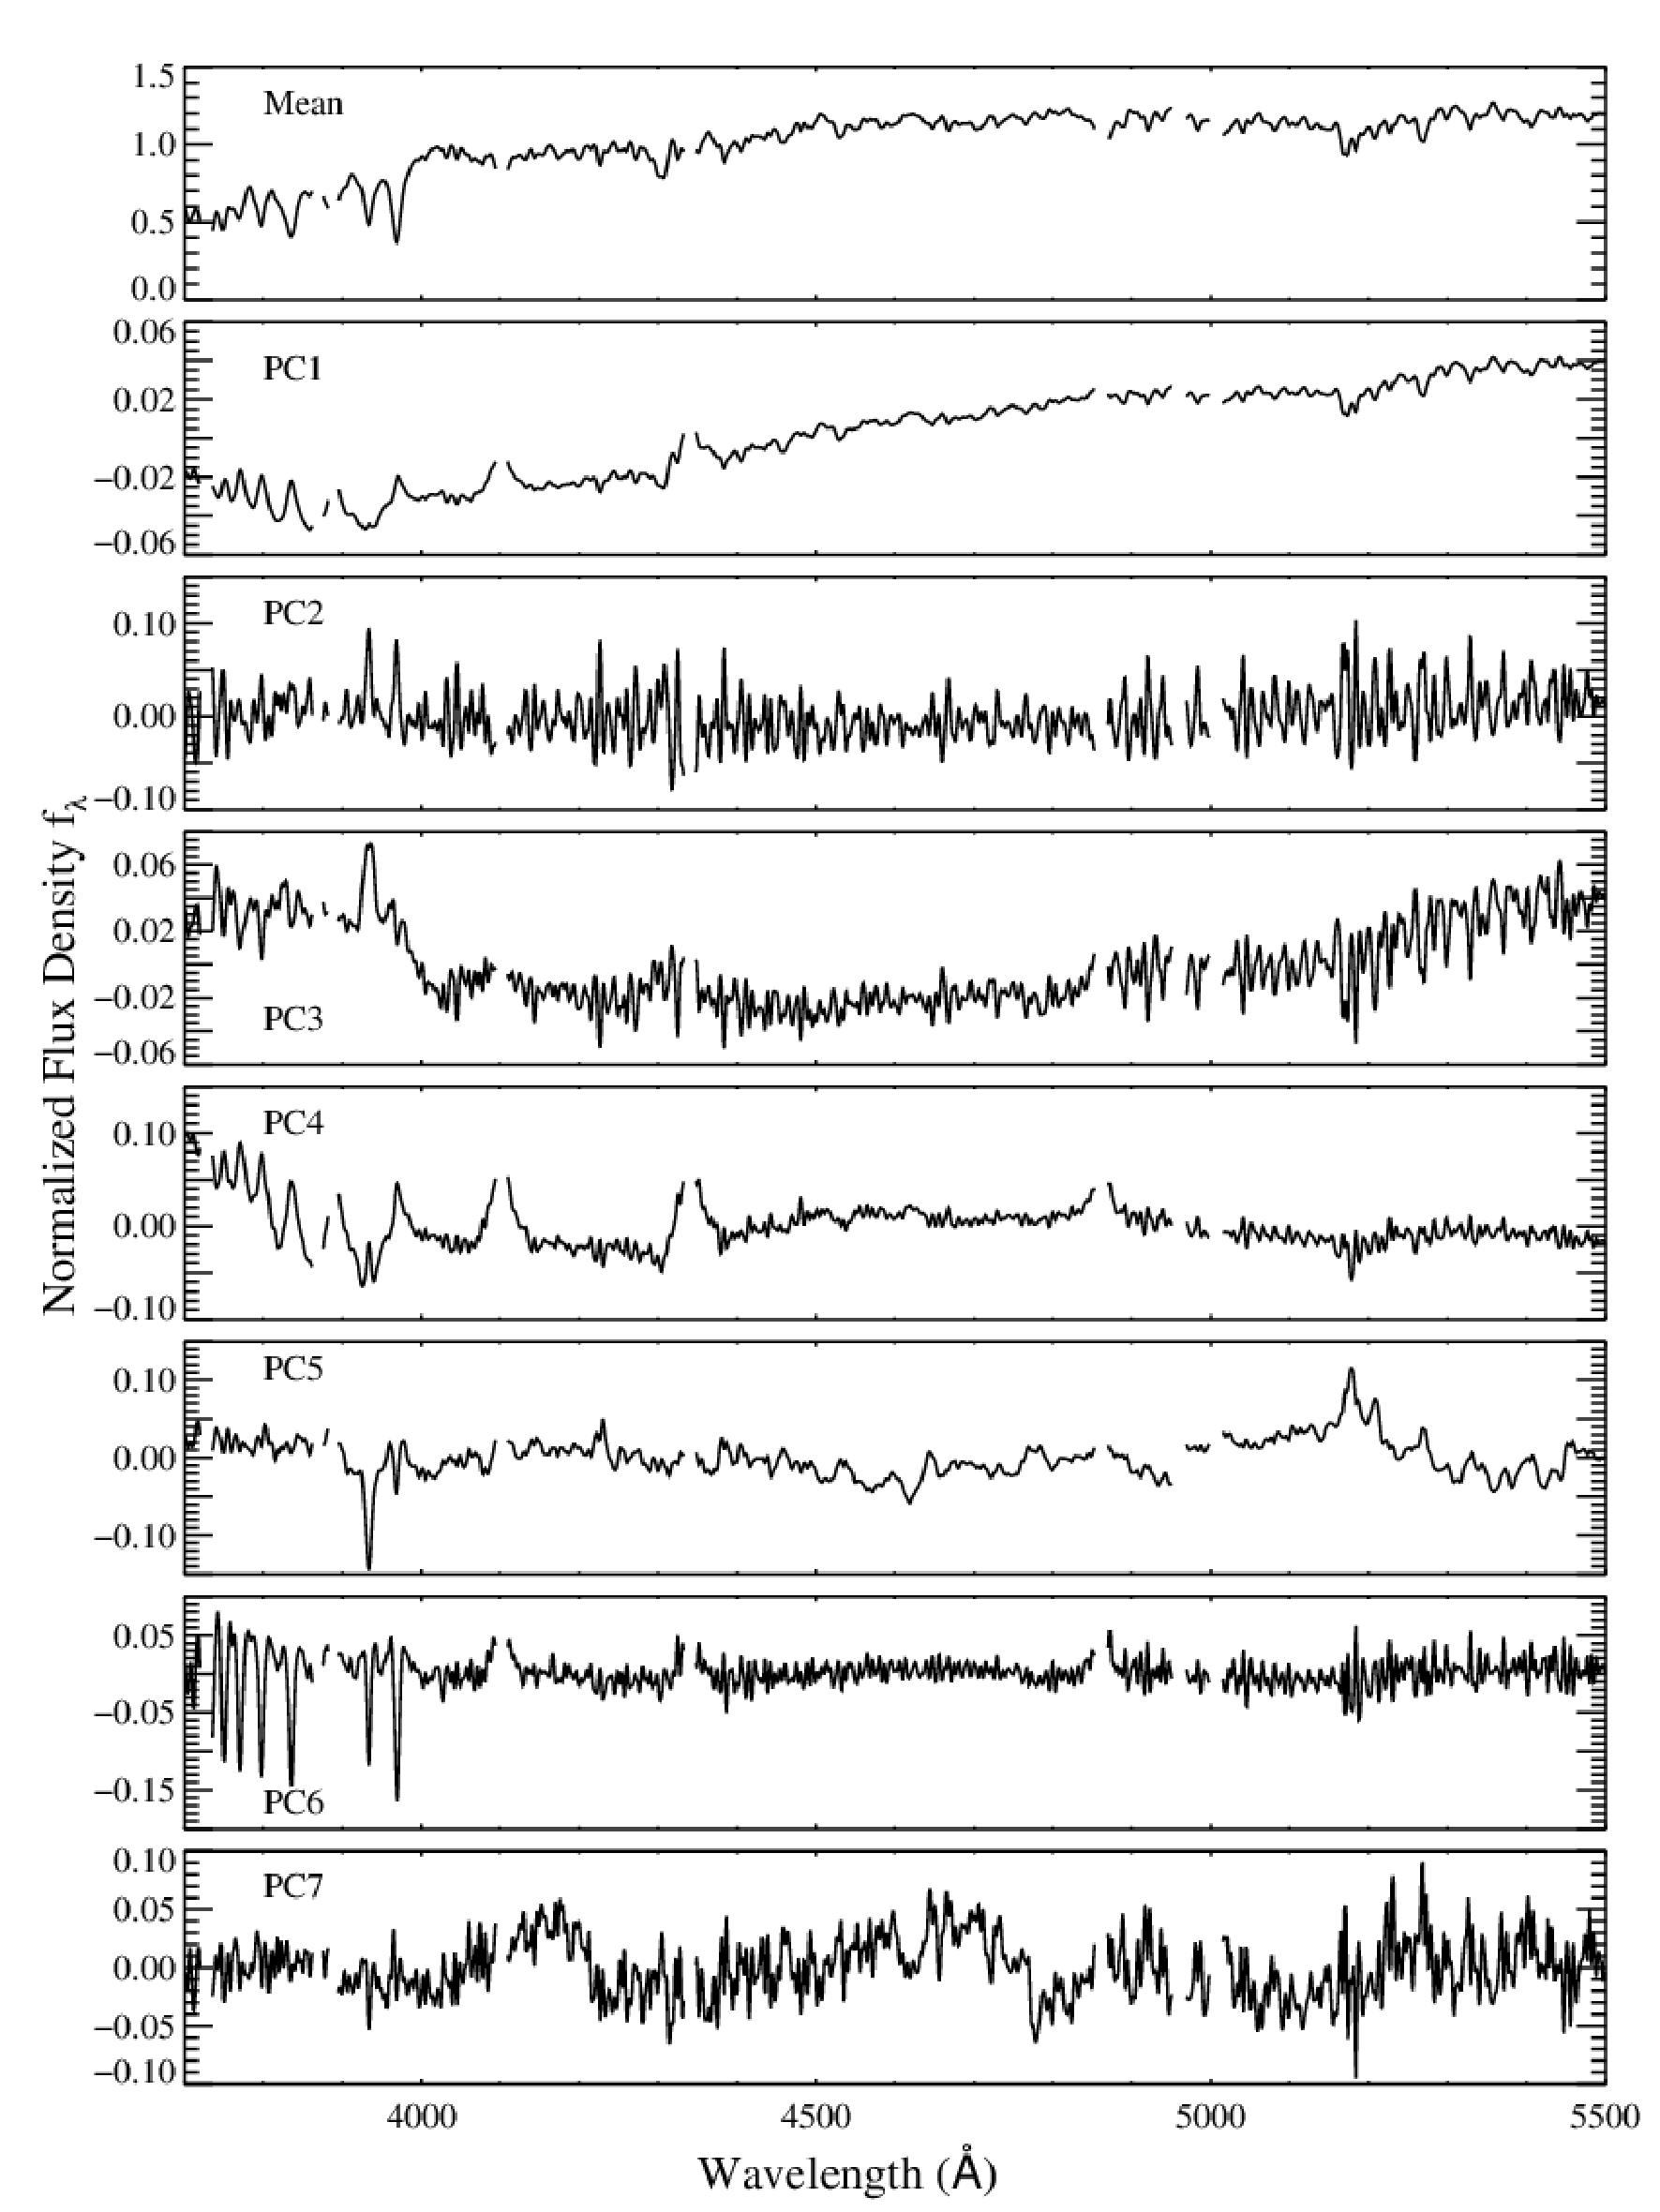
\includegraphics[height=0.8\textwidth]{figuras/figChen2012fig2.pdf}
    \caption[]{De cima para baixo: O espectro médio da biblioteca de espectros modelos seguido dos sete primeiros autoespectros da análise PCA.
    Retirado de \citet{Chen2012}.}
    \label{fig:Chen2012fig2}
    \end{center}
\end{figure}

\section{Objetivos}
O objetivo principal desse trabalho é avançar nossas análises estatísticas nos cubos de dados de galáxias do Projeto CALIFA {\em Survey}, procurando
padrões tanto em dimensão espectral, quanto espacial. Pretendemos:
\begin{itemize}
  \item Aplicar a tomografia PCA aos mais recentes cubos de espectros observados das galáxias do CALIFA, e nos anteriores agora em sua nova versão;
  \item Procurar sentido físico nas componentes principais e seus respectivos tomogramas, bem como procurar possíveis correlações entre resultados
  para diferentes tipos morfológicos, massas, etc;
  \item Análisar e comparar o efeito da aplicação da tomografia PCA nos cubos de espectros resultantes da síntese de populações estelares (espectros
  sintéticos) feita com o \starlight.
  \item Explorar a aplicação de filtros espectrais e espaciais baseados em PCA e outras técnicas ({\em wavelets}, {\em
  fourier}, distâncias em diferentes espaços, clusterização, etc.).
\end{itemize}

\section{Metodologia}
Através de nossa parceria com os pesquisados do IAA, na Espanha, possuimos um ambiente perfeito para o desenvolvimento desse projeto. Descrevemos aqui
nossa metodologia proposta para tal fim.

\subsection{O projeto CALIFA e o Instituto de Astrofísica de Andalucía}

O CALIFA foi concebido para que seu legado seja abrangente, possibilitando diversos tipos de estudos em diversas áreas. Para esta finalidades, está
observando $\sim 600$ galáxias com um campo de visão de $\sim1.3$ arcmin$^2$ em duas configurações que cobrem a janela espectral de 3650-7000 \AA. Sua
amostra cobre o diagrama cor-magnitude (Figura \ref{fig:cm-uzMz}) e diversos tipos morfológicos. Existem alguns poucos {\em surveys} de IFU e todos
com, além de poucos objetos e campo de visão menor que o CALIFA, focos de estudo mais estreitos, dificultando o legado do {\em survey} para pequisas
científicas mais abrangentes \citep[SAURON;][região central de 72 galáxias com $z < 0.01$.]{de-Zeeuw2002} \citep[PINGS;][algumas galáxias muito
próximas ($\sim 10$ Mpc) e o estudo atual de 70 (U)LIRGs com $z <0.26$]{RosalesOrtega2010} \citep[VENGA;][$30$ galáxias espirais]{Blanc2010}
\citep[ATLAS\textsuperscript{3D};][260 galáxias {\em early-type} próximas]{Cappellari2011}. Outros {\em surveys} IFU ainda estão por vir, como SAMI
\citep{Croom2012} e MaNGA\footnote{\url{http://www.sdss3.org/future/manga.php}}.

Devido a participação direta e intensa dos pesquisadores da UFSC e do IAA dentro do projeto CALIFA, essa parceria é o ambiente propício para levar
adiante este estudo, com laboratórios próprios e {\em hardware} suficientes para o avanço de nosso projeto. No IAA se encontram muitos pesquisadores
participantes do Projeto CALIFA, portanto, funciona como centro físico de pesquisadores do projeto, além de contar com a pesquisadora Rosa M. González
Delgado, uma das principais líderes do projeto que também atua como Pesquisadora Visitante do Exterior (PVE-CsF) aqui na UFSC. Rubén García Benito,
que faz parte do grupo de redução dos dados do CALIFA, e Enrique Pérez, do grupo de populações estelares, já trabalham em nossa parceria e possuem
domínio de técnicas exploradas por nosso projeto.

\begin{figure}
	\begin{center}
    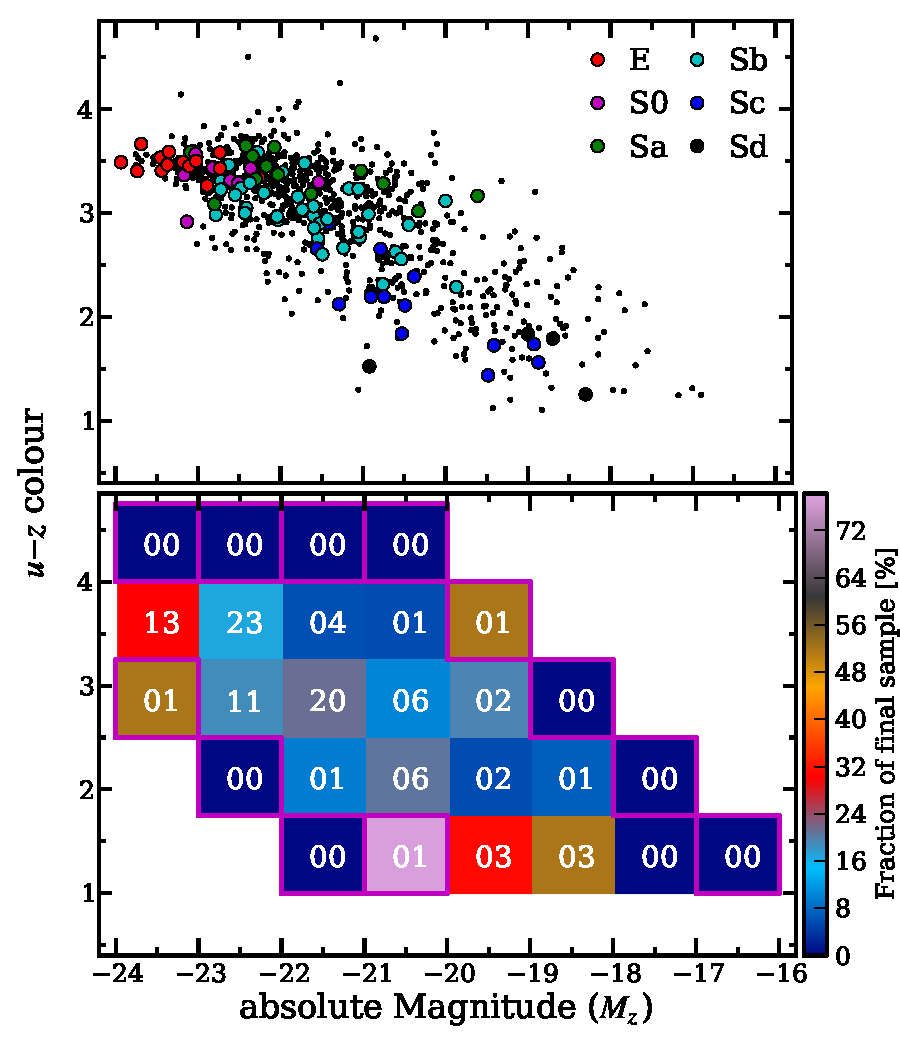
\includegraphics[height=0.5\textwidth]{figuras/figHusemann2013Fig2.pdf}
    \caption[Diagrama cor-magnitude para as galáxias do CALIFA.]
    {Distribui\c{c}\~ao das galáxias do CALIFA no diagrama cor magnitude $u-z$ vs. $M_z$. {\em Painel superior}: Em pontos pretos est\~ao as galáxias
    pertencente a amostra-m\~ae e em cores as galáxias presentes no CALIFA DR1. As diferentes cores representam os diferentes tipos morfológicos.
    {\em Painel inferior}: A fra\c{c}\~ao de galáxias observadas pelo DR1 em rela\c{c}\~ao a amostra-m\~ae. Retirado de \citet{Husemann2013}.}
    \label{fig:cm-uzMz}
    \end{center}
\end{figure}

\begin{figure}
	\begin{center}
    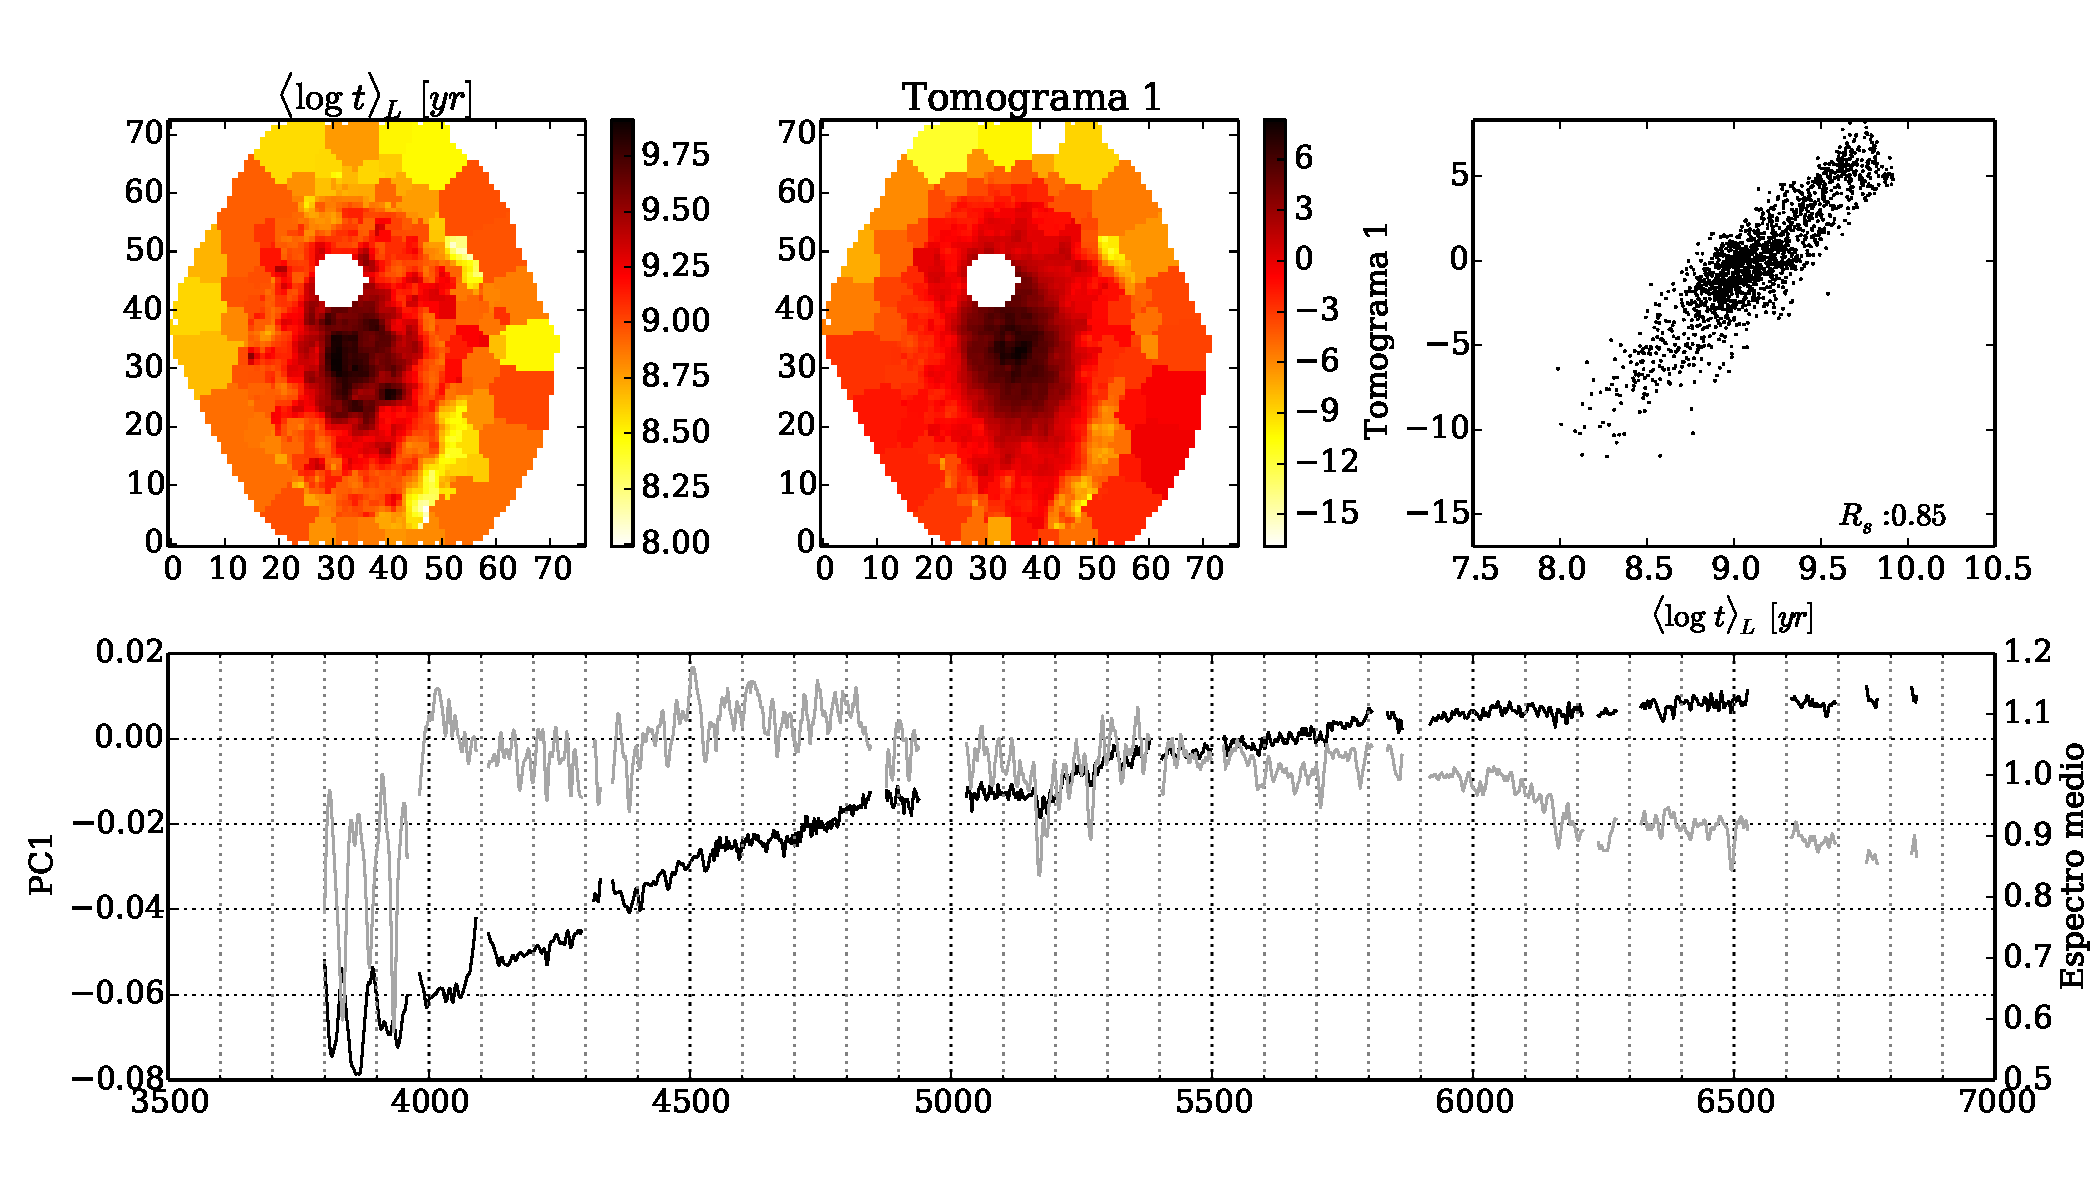
\includegraphics[width=0.85\textwidth]{figuras/K0277-f_obs_norm_pc_1_prop_0.pdf}
    \caption[]{Correla\c{c}\~ao entre a idade estelar média ponderada pela luz (\meanL{\log\ t}) e o tomograma 1 para a galáxia NGC 2916 (CALIFA 277).
    {\em Paineil superior esquerdo}: Distribui\c{c}\~ao espacial da idade estelar média ponderada pela luz. {\em Painel superior central}:
    Tomograma da componente principal 1 (PC1). {\em Painel superior direito}: Correla\c{c}\~ao entre \meanL{\log\ t} e o tomograma 1. Destaque para o
    coeficiente de correla\c{c}\~ao de Spearman no canto inferior direito. {\em Painel inferior:} Componente principal 1 juntamente com o espectro
    médio ({\em eixo direito}).}
    \label{fig:K0277corre}
    \end{center}
\end{figure}

\subsection{\pycasso e \pcalifa}

A sintese espectral de uma galáxia do CALIFA gera um número muito grande de resultados. Cada espectro de entrada para a síntese pertence a uma posição
determinada ({\em spaxel}\footnote{{\em Spaxel} vem de {\em Spectral pixel}. Um {\em spaxel} é um píxel com três dimensões (x, y, $\lambda$)}) da
galáxia, resultando assim em para as propriedades físicas e medidas de extinção estelares com dimensão espacial. Para organização desses resultados,
que necessitam ser armazenadas com as informações originais dos cubos, André L. de Amorim, juntamente com outros colaboradores de nosso grupo e do
projeto CALIFA, construiu o programa \pycasso ({\em Python CALIFA \starlight Synthesis Organizer}, descrito na sec. 4 de \citet{CidFernandes2013})
para tal função. O \pycasso organiza os resultados da síntese de populações estelares e demais dados provenientes de outros programas pertencentes ao
{\em pipeline} do CALIFA. Esses programas fazem a redução dos espectros, definição de máscaras espaciais e espectrais (remoção de objetos espúrios,
marcação de {\em spaxels} problemáticos), entre outros. Este programa facilita muito toda a ciência exploratória nos cubos de espectros do CALIFA.

Em minha dissertação de mestrado desenvolvemos um programa chamado de \pcalifa, que utiliza o \pycasso como biblioteca e os cubos de espectros do
CALIFA para o cáculo das componentes principais e dos tomogramas PCA. Encontramos diversas correlações entre a distribuição espacial das componentes e
os tomogramas PCA. Um exemplo pode ser visto na Figura \ref{fig:K0277corre} onde encontramos a uma ótima correlação entre a idade estelar média
ponderada pela luz (\meanL{\log\ t}) e o tomograma 01. Essas correlações formam uma certa engenharia reversa no sentido de buscar os parâmetros mais
``importantes'' em variância (as PCs) que mapeiam propriedades físicas, de uma forma não-paramétrica. Os estudos iniciais e exploratórios realizados
no mestrado devem agora ser retomados de forma mais completa e sistemática no doutorado.

\subsection{Explorando as características de filtragem dos dados com tomografia PCA e wavelets}

Utilizando tomografia PCA pode-se reconstruir os espectros originais criando combinações dos elementos da base ortonormal, ordenados pela variância,
resultante da técnica (componentes principais). O cubo de espectros pode ser reconstruído  ($\mathbf{F}_{z \lambda}^{rec}$) usando os tomogramas
($\mathbf{T}{}_{z k}$), os autovetores ($\mathbf{E}{}_{\lambda k}$) e o espectro médio ($\mean{\mathbf{F}_\lambda}$) através da equação:
\begin{equation}
	\mathbf{F}{}_{z \lambda}^{rec} = \mathbf{T}{}_{z k}(r \leq k) \cdot [\mathbf{E}{}_{\lambda k}(r \leq k)]^T + \mean{\mathbf{F}_\lambda}
\end{equation}
\noindent onde utiliza-se $r \leq k$ autoespectros ($k$ é o número total de autovetores). O índice $z$ designa uma zona da galáxia. 

Todo o processo de obtenção e redução dos dados com IFS adiciona ``ruído'' no sinal obtido. Padrões inseridos nos dados que podem atrapalhar na
interpretação dos resultados de qualquer análise. Esses ruídos se espalham em padrões espectrais e padrões espaciais. Usando PCA dos espectros esses
elementos geralmente são encontrados em componentes com variancia mais baixa. Como citado anteriormente, em \citet{Riffel2011} podemos ver o uso da
Transformada {\em Wavelet} Discreta ({\em Discrete wavelet transform} - DWT) juntamente com tomografia PCA para filtragem de cubos de dados IFS.
Para cada imagem em determinado comprimento de onda (cada comprimento de onda em um cubo de dados forma uma imagem) aplica-se a DWT e depois a
tomografica PCA para cada {\em wavelet}, obtendo assim um filtro de características espaciais. Nesse caso os dados são do {\em Gemini Near-infrared
Integral Field Spectrograph} (NIFS) para a galáxia NGC 591. Os campos de visão do Gemini e do CALIFA são completamente diferentes. Praticamente cada
elemento de resolução do CALIFA é um campo inteiro do Gemini, fazendo com que nossa análise seja pioneira para cubos de dados abrangendo galáxias
inteiras. Outras técnicas com medidas de distâncias em espaços multidimensionais, clusterização, entre outras, serão análisadas, a fim de se encontrar
padrões pertinentes nos dados.

% bibliografia
\bibliographystyle{apj}
\bibliography{apj-jour,bibliografia}
    
\end{document}
